%============================================================
%  Silver Gjeka — Curriculum Vitae (versione Italiana)
%  Header Layout: Foto a sinistra, Nome e Contatti a destra
%============================================================
\documentclass[a4paper,11pt]{article}

\usepackage[T1]{fontenc}
\usepackage[utf8]{inputenc}
\usepackage[italian]{babel}
\usepackage{mathptmx}                 % Font Times-like
\usepackage[top=0.7in,bottom=0.7in,left=0.85in,right=0.85in]{geometry}
\usepackage{enumitem}
\usepackage{tabularx}
\usepackage{graphicx}
\usepackage[hidelinks]{hyperref}

\pagestyle{empty}
\setlength{\parindent}{0pt}
\setlist[itemize]{leftmargin=1.5em,itemsep=1.5pt,topsep=2pt,parsep=0pt,label=\textbullet}

% ---- linea puntinata sottile ----
\newcommand{\dsep}{\par\vspace{3pt}%
  \noindent\hbox to \linewidth{\leaders\hbox to 4.5pt{\hss\textperiodcentered\hss}\hfill}%
  \par\vspace{3pt}}

% ---- intestazione di sezione centrata e maiuscola ----
\newcommand{\cvsec}[1]{\dsep{\centering\large\MakeUppercase{#1}\par}\vspace{3pt}}

% ---- riga "Titolo .......... allineato a destra" ----
\newcommand{\entry}[2]{\textbf{#1}\hfill\textbf{#2}\par}

% ---- riga progetto compatta ----
\newcommand{\proj}[3]{\textbf{#1}: #2 \textit{(#3)}\par\smallskip}

\begin{document}

%====================== INTESTAZIONE (FOTO A SINISTRA, TESTO A DESTRA) ======================
\noindent
\begin{minipage}[t]{0.22\textwidth}
  \vspace{0pt}
  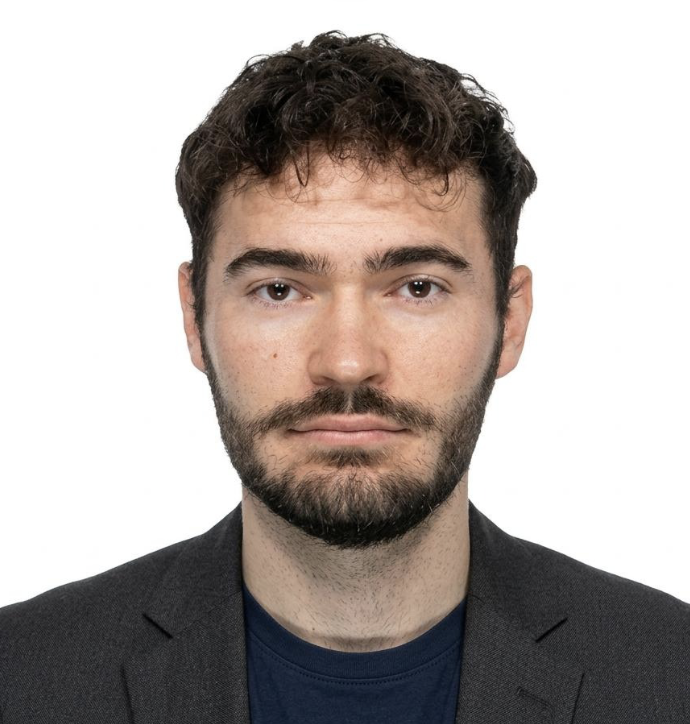
\includegraphics[width=3.1cm, height=3.6cm, keepaspectratio]{photo.png}
\end{minipage}%
\begin{minipage}[t]{0.78\textwidth}
  \vspace{0pt}
  \raggedright
  {\fontsize{24}{28}\selectfont\bfseries Silver Gjeka}\\[8pt]
  \begin{tabular}{@{}l@{\hspace{8pt}}l@{}}
    \textbf{Telefono:} & (+39) 351 6091609 \\[2pt]
    \textbf{Email:}    & \href{mailto:silvergjeka@gmail.com}{silvergjeka@gmail.com} \\[2pt]
    \textbf{GitHub:}   & \href{https://github.com/silvergjeka22}{github.com/silvergjeka22} \\[2pt]
    \textbf{LinkedIn:} & \href{https://www.linkedin.com/in/silver-gjeka-56b9931a4/}{linkedin.com/in/silver-gjeka-56b9931a4} \\[2pt]
    \textbf{Luogo:}    & Verona, Italia
  \end{tabular}
\end{minipage}

\vspace{12pt}

%====================== TITOLO + PROFILO ======================
\cvsec{Sviluppatore Software \& AI}

Laureato in Informatica e studente magistrale in Intelligenza Artificiale presso l'Università degli Studi di Verona, unisco solide basi di ingegneria del software a un portfolio consolidato in machine learning, deep learning e computer vision. Con esperienza come full-stack developer, sviluppo applicazioni concrete e orientate ai dati, dal modello all'interfaccia. Motivato, curioso e desideroso di crescere all'interno di un team di sviluppo software o AI.

%====================== ISTRUZIONE ======================
\cvsec{Istruzione}

\entry{Università degli Studi di Verona: Laurea Magistrale in Intelligenza Artificiale}{2024 -- Presente}
Percorso magistrale incentrato su machine learning, deep learning, computer vision ed elaborazione del linguaggio naturale, unendo solide basi teoriche a progetti pratici di intelligenza artificiale. \textit{Voto finale: in corso.}

\vspace{6pt}
\entry{Università degli Studi di Verona: Laurea Triennale in Informatica}{2020 -- 2024}
\textit{Tesi:} ``Sviluppo di una web app per il monitoraggio dell'uptime e della sicurezza degli IP''.

%====================== ESPERIENZA PROFESSIONALE ======================
\cvsec{Esperienza Professionale}

\entry{BSQ: Verona, Italia}{2023 -- 2024}
\textbf{Full Stack Developer}\par
Ho progettato e sviluppato, dall'inizio alla fine, una web app sicura per il monitoraggio dell'uptime e della sicurezza dei dispositivi IP: realizzata come tesi di laurea triennale, lavorando in autonomia sull'intero stack.
\begin{itemize}
  \item Scansioni di rete asincrone con Celery e Nmap (porte aperte, identificazione del sistema operativo, controlli di sicurezza) con notifiche immediate delle minacce.
  \item Dashboard interattiva con geolocalizzazione su mappa, monitoraggio in tempo reale dei dispositivi attivi/inattivi e tabella ricercabile.
  \item Autenticazione sicura, gestione dei permessi per ruolo (utente/admin) e supporto multilingua, con database MySQL.
  \item Tecnologie: Python, Flask, Django, Celery, Nmap, MySQL, HTML, CSS, JavaScript, Bootstrap.
\end{itemize}

\vspace{6pt}
\entry{Compass Group: Verona, Italia}{Giu 2022 -- Set 2022}
\textbf{Barman}\par
\begin{itemize}
  \item Servizio al cliente in un ambiente dinamico; capacità di comunicazione, lavoro di squadra e gestione del tempo.
\end{itemize}

%====================== PROGETTI ======================
\cvsec{Progetti}

\proj{Rilevamento di Fratture Ossee con Explainable AI}{Classificatore ResNet18 su radiografie la cui attenzione Grad-CAM si allinea alle annotazioni dei radiologi, con una pipeline YOLOv8 + classificatore che raggiunge il 93\% di accuratezza.}{Python, PyTorch}
\proj{Visual Question Answering (VQA)}{Modelli multimodali che rispondono a domande in linguaggio naturale sulle immagini, con il confronto di 8 architetture visione--linguaggio (CLIP, ResNet, BERT, LSTM).}{Python, PyTorch, Transformers}
\proj{Guida Sicura Neuro-Simbolica}{Agenti di reinforcement learning (DQN, PPO) resi più sicuri con regole del codice stradale in logica temporale, riducendo gli incidenti dal 35\% al 5\% in un simulatore mai visto.}{Python, RL}
\proj{Lifelong Action Learning}{Riconoscitore di azioni da video (CNN + LSTM) su UCF101 che apprende nuove azioni nel tempo senza dimenticare, con replay, distillazione e meta-learning MAML.}{Python, PyTorch}
\proj{MACURA Drone Racing}{Addestramento di un drone simulato a gareggiare su un percorso 3-D con vento, confrontando metodi di reinforcement learning model-based (MACURA, MBPO, M2AC, SAC).}{Python, MuJoCo}
\proj{Riconoscimento di Attività Fisiche}{Pipeline di machine learning end-to-end che classifica sei esercizi in palestra da dati di accelerometro/giroscopio; il modello migliore (Random Forest) raggiunge il 98.3\%.}{Python, scikit-learn}
\proj{CongruentClosureDAG}{Algoritmo di congruence closure basato su DAG per la soddisfacibilità di formule di uguaglianza con array, liste e funzioni non interpretate, con visualizzatore grafico.}{Java}

\smallskip
\textbf{Altri progetti:} il portfolio completo di AI e software è su \href{https://github.com/silvergjeka22}{github.com/silvergjeka22}.

%====================== COMPETENZE TECNICHE ======================
\cvsec{Competenze Tecniche}

\textbf{Linguaggi:} Python, Java, C, JavaScript, Swift, MATLAB \\[3pt]
\textbf{AI / ML:} PyTorch, scikit-learn, Hugging Face Transformers, Computer Vision, Deep Learning, NLP, Reinforcement Learning, Explainable AI \\[3pt]
\textbf{Web:} Flask, Django, HTML, CSS, Bootstrap \\[3pt]
\textbf{Dati \& Strumenti:} MySQL, pandas, NumPy, Celery, Nmap, Git/GitHub, LaTeX

%====================== LINGUE ======================
\cvsec{Lingue}

\begin{tabularx}{\textwidth}{*{3}{>{\centering\arraybackslash}X}}
\textbf{Albanese}: Madrelingua & \textbf{Italiano}: C1 & \textbf{Inglese}: B2 \\
\end{tabularx}

%====================== ALTRO ======================
\cvsec{Altro}

\textbf{Programmi:} CyberChallenge.IT 2026, programma nazionale di formazione in cybersecurity. \\[3pt]
\textbf{Open Badge:} Sviluppo iOS con Swift; Problem Solving e Soft Skills (Università degli Studi di Verona, 2022).

%====================== COMPETENZE PRINCIPALI ======================
\cvsec{Competenze Principali}

\begin{tabularx}{\textwidth}{*{3}{>{\centering\arraybackslash}X}}
Machine Learning        & Deep Learning            & Computer Vision         \\[4pt]
Sviluppo Full-Stack     & Analisi dei Dati         & Problem Solving         \\[4pt]
Elaborazione del Linguaggio & Lavoro di Squadra    & Apprendimento Rapido    \\
\end{tabularx}

%====================== REFERENZE ======================
\cvsec{Referenze}

Disponibili su richiesta.

\vspace{6pt}
{\footnotesize Autorizzo il trattamento dei miei dati personali contenuti nel presente CV ai sensi del Regolamento UE 2016/679 (GDPR) e del D.Lgs. 196/2003.\par}

%====================== FIRMA ======================
\vspace{22pt}
\begin{flushright}
{\itshape\Large Silver Gjeka}\\[6pt]
\rule{5.5cm}{0.4pt}\\
{\footnotesize Firma}
\end{flushright}

\end{document}